\section{Experimental Evaluation}

In this section we compare our model to previous methods on a rich set of experiments. The code and further supplementary material is available online (\url{www.daml.in.tum.de/postnet}).

\textbf{Baselines.} We have special focus on comparing with other models parametrizing Dirichlet distributions. We use Prior Networks (PN) trained with KL divergence (\textbf{KL-PN}) \cite{prior_net} and Reverse KL divergence (\textbf{RKL-PN}) \cite{rev_kl_prior_net}. These methods assume the knowledge of in- and out-of-distribution samples. For fair evaluation, the actual OOD test data cannot be used; instead, we used uniform noise on the valid domain as OOD training data. Additionally we trained RKL-PN with FashionMNIST as OOD data for MNIST (\textbf{RKL-PN w/ F.}). We also compare to Distribution Distillation (\textbf{Distill.}) \cite{distribution_distillation}, which learns Dirichlet distributions with maximum likelihood by using soft-labels from an ensemble of networks. 
As further baselines, we compare to dropout models (\textbf{Dropout Net}) \cite{drop_out} and ensemble methods (\textbf{Ensemble Net}) \cite{ensemble_simple}, which are state of the art in many tasks involving uncertainty estimation \cite{uncertainty_survey}. Empirical estimates of the mean and variance of \smash{$q\dataix$} are computed based on the neuron drop probability $p_{\text{drop}}$, and $m$ individually trained networks for ensemble.

All models share the same core architecture using 3 dense layers for tabular data, and 3 conv. + 3 dense layers for image data. Similarly to \cite{prior_net, rev_kl_prior_net}, we also used the VGG16 architecture \cite{vgg} on CIFAR10. We performed a grid search on $p_{\text{drop}}$, $m$, learning rate and hidden dimensions, and report results for the best configurations. Results are obtained from 5 trained models with different initializations.
Moreoever, for all experiments, we split the data into train, validation and test set  ($60\%$, $20\%$, $20\%$) and train/evaluate all models on $5$ different splits. Besides the mean we also report the standard error of the mean. Further details are given in the appendix.

\textbf{Datasets.} We evaluate on the following real-world datasets: \textbf{Segment} \cite{uci_datasets}, \textbf{Sensorless Drive} \cite{uci_datasets}, \textbf{MNIST} \cite{mnist} and \textbf{CIFAR10} \cite{cifar10}. The former two datasets (Segment and Sensorless Drive) are tabular datasets with %unbounded input domain of 
dimensionality 18 and 49 and with 7 and 11 classes, respectively. We rescale all inputs between $[0, 1]$ by using the $\min$ and $\max$ value of each dimension from the training set. Additionally, we compare all models on 2D synthetic data composed of three Gaussians each. Datasets are presented in  more detail in the appendix.

\textbf{Uncertainty Metrics.} We follow the method proposed in \cite{uncertainty_survey} and evaluate the coherence of confidence, uncertainty calibration and OOD detection. Note that our goal is not to improve accuracy; still we report the numbers in the experiments.

\underline{Confidence calibration:} We aim to answer `\textit{Are more confident (i.e. less uncertain) predictions more likely to be correct?}'. We use the area under the precision-recall curve (AUC-PR) to measure confidence calibration. For aleatoric confidence calibration (\textbf{Alea. Conf.}) we use \smash{$\underset{\iclass}{\max} \; \bar{\vect{p}}_\iclass\dataix$} as the scores with labels 1 for correct and 0 for incorrect predictions. For epistemic confidence calibration (\textbf{Epist. Conf.}), we distinguish Dirichlet-based models, and dropout and ensemble models. For the former we use \smash{$\underset{\iclass}{\max}\; \bm{\alpha}_\iclass\dataix$} as scores, and for the latter we use the (inverse) empirical variance \smash{$\tilde{\vect{p}}_c\dataix$} of the predicted class, estimated from 10 samples.

\underline{Uncertainty calibration:} We used Brier score (\textbf{Brier}), which is computed as \smash{$\frac{1}{N}\sum_{i}^N \|\bar{\vect{p}}\dataix - \vect{y}\dataix\|_2$}, where $\vect{y}\dataix$ is the one-hot encoded ground-truth class of data point $i$. For Brier score, lower is better.

\underline{OOD detection:} Our main focus lies on the models' ability to detect out-of-distribution samples. We used AUC-PR to measure performance. For aleatoric OOD detection (\textbf{Alea. OOD}), the scores are \smash{$\underset{\iclass}{\max} \; \bar{\vect{p}}_\iclass\dataix$} with labels 1 for ID data and 0 for OOD data. Fo epistemic OOD detection (\textbf{Epist. OOD}), the scores for Dirichlet-based models are given by \smash{$\alpha_0\dataix = \sum_\iclass \alpha_\iclass\dataix$}, while we use the (inverse) empirical variance \smash{$\tilde{\vect{p}}\dataix$} for ensemble and dropout models. To provide a comprehensive overview of OOD detection results we use different types of OOD data as described below. 

\textit{Unseen datasets.} We use data from other datasets as OOD data for the image-based models. We use data from FashionMNIST \cite{fashionmnist} and K-MNIST \cite{kmnist}  as OOD data for models trained on MNIST, and data from SVHN \cite{svhn} as OOD for CIFAR10.

\textit{Left-out classes.} For the tabular datasets (Segment and Sensorless Drive) there are no other datasets that are from the same domain. To simulate OOD data we remove one or more classes from the training data and instead consider them as OOD data. We removed one class (class sky) from the Segment dataset and two classes from Sensorless Drive (class 10 and 11).

\textit{Out-of-domain.} In this novel evaluation we consider an extreme case of OOD data for which the data comes from different value ranges (\textbf{OODom}). E.g., for images we feed unscaled versions in the range $[0, 255]$ instead of scaled versions in $[0,1]$. We argue that models should easily be able to detect data that is extremely far from the data distribution. However, as it turns out, this is surprisingly difficult for many baseline models.

\textit{Dataset shifts.} Finally, for CIFAR10, we use 15 different image corruptions at 5 different severity levels \cite{benchmarking_corruptions}. This setting evaluates the models' ability to detect low-quality data (Fig.~\ref{cifar_shifts}b,c).

\begin{table}
    \centering
    \resizebox{.9 \textwidth}{!}{%
\begin{tabular}{lllllll}
\toprule
{} &  \textbf{Acc.} & \textbf{Alea. Conf.} & \textbf{Epist. Conf.} & \textbf{Brier} & \textbf{OOD Alea.} & \textbf{OOD Epist.} \\
\midrule
\midrule
\textbf{Drop Out  } &  89.32$\pm$0.2 &        98.21$\pm$0.1 &         95.24$\pm$0.2 &  28.86$\pm$0.4 &      35.41$\pm$0.4 &       40.61$\pm$0.7 \\
\textbf{Ensemble  } &  99.37$\pm$0.0 &        99.99$\pm$0.0 &         *99.98$\pm$0.0 &   2.47$\pm$0.1 &      50.01$\pm$0.0 &       50.62$\pm$0.1 \\
\midrule
\textbf{Distill.  } &  93.66$\pm$1.5 &        98.29$\pm$0.5 &         98.15$\pm$0.5 &  44.94$\pm$1.4 &       32.1$\pm$0.6 &       31.17$\pm$0.2 \\
\textbf{KL-PN     } &  94.77$\pm$0.9 &        99.52$\pm$0.1 &         99.47$\pm$0.1 &  21.47$\pm$1.9 &      35.48$\pm$0.8 &        33.2$\pm$0.6 \\
\textbf{RKL-PN    } &  99.42$\pm$0.0 &        99.96$\pm$0.0 &         99.89$\pm$0.0 &   9.07$\pm$0.1 &      45.89$\pm$1.6 &       38.14$\pm$0.8 \\
\textbf{PostN Rad.} &  98.02$\pm$0.1 &        99.89$\pm$0.0 &         99.47$\pm$0.0 &   5.51$\pm$0.2 &      72.89$\pm$0.8 &       \textbf{*88.73$\pm$0.5} \\
\textbf{PostN IAF } &  \textbf{*99.52$\pm$0.0} &        \textbf{*100.0$\pm$0.0} &         \textbf{99.92$\pm$0.0}&   \textbf{*1.43$\pm$0.1} &      \textbf{*82.96$\pm$0.8} &       88.65$\pm$0.4 \\
\bottomrule
\end{tabular}

    }
    \caption{Results on Sensorless Drive dataset. Bold numbers indicate best score among Dirichlet parametrized models and starred numbers indicate best scores among all models.}
    \label{fig:unc_sensorless_drive}
%\vspace{-.0cm}
\end{table}

\textbf{Results.} 
Results for the Sensorles Drive dataset are shown in Tab.~\ref{fig:unc_sensorless_drive}. Tables for other datasets are in the appendix. Even without requiring expensive sampling, \oursacro performs on par for accuracy and confidence scores with other models, brings a significant improvement for calibration within the Dirichlet-based models, and outperforms all other models by a large margin (more than $+30\%$ abs. improvement) for OOD detection. Radial flow and IAF variants both achieve strong performance for all datasets (see app.). We use the smaller model (i.e. Radial flow) for comparison in the following. In our experiments, note that using one Radial flow per class represents a small overhead of only $80$ parameters per class, which is negligible compared to the encoder architectures (e.g. VGG16 has 138M parameters).

\begin{figure}
    \centering
    \begin{subfigure}[t]{0.33 \textwidth}
        \centering
        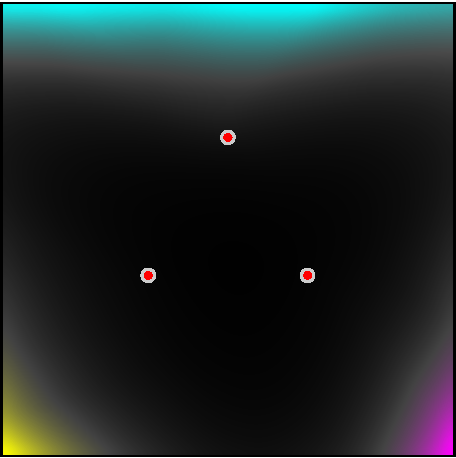
\includegraphics[width=0.5 \textwidth]{sections/006_neurips2020/figures/three_gaussians_no_flow-crop.pdf}
        \caption{\oursacro: \NoFlow}
    \end{subfigure}%   
    \begin{subfigure}[t]{0.33 \textwidth}
        \centering
        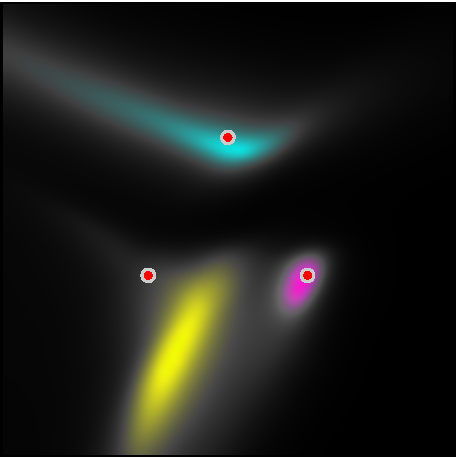
\includegraphics[width=0.5 \textwidth]{sections/006_neurips2020/figures/three_gaussians_no_UCE-crop.pdf}
        \caption{\oursacro: \NoUCE}
    \end{subfigure}%   
    \begin{subfigure}[t]{0.33 \textwidth}
        \centering
        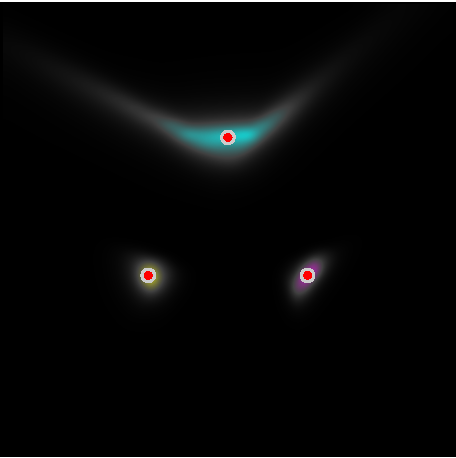
\includegraphics[width=0.5 \textwidth]{sections/006_neurips2020/figures/three_gaussians_normal-crop.pdf}
        \caption{\oursacro: Complete}
    \end{subfigure}%

    \caption{Uncertainty visualization for a 2D 3-Gaussians dataset. Red dots indicate the Gaussians means. Darker regions indicate high epistemic uncertainty for a class prediction. Ablated models fail even a simple dataset while \oursacro shows high certainty around gaussians means only.}
    \label{fig:toy_ablation}
	%\vspace{-.0cm}
\end{figure}

\begin{table}[H]
\resizebox{1 \textwidth}{!}{%
\begin{tabular}{lllllll}
\toprule
{} &  \textbf{Acc.} & \textbf{Alea. Conf.} & \textbf{Epist. Conf.}  & \textbf{Brier} & \textbf{OOD Alea.} & \textbf{OOD Epist.} \\
\midrule
\midrule
\textbf{PostN: No-Flow        } &  \cellcolor{Gray} 55.38$\pm$0.7 & \cellcolor{Gray} 85.46$\pm$0.3 & \cellcolor{Gray} 82.58$\pm$0.6 & \cellcolor{Gray} 64.4$\pm$0.6 & \cellcolor{Gray} 29.59$\pm$0.1 & \cellcolor{Gray} 31.15$\pm$0.4 \\
\textbf{PostN: No-Bayes-Loss} &   96.6$\pm$0.2 & 99.74$\pm$0.0 & 98.68$\pm$0.1 & \cellcolor{Gray} 8.85$\pm$0.4 & \cellcolor{Gray} 62.39$\pm$1.5 & \cellcolor{Gray} 82.63$\pm$1.4 \\
\textbf{PostN: Seq-No-Bn   } &  \cellcolor{Gray} 15.09$\pm$1.0 & \cellcolor{Gray} 39.88$\pm$7.2 &  \cellcolor{Gray}  39.86$\pm$7.2 &  \cellcolor{Gray} 89.88$\pm$1.3 & \cellcolor{Gray} 57.19$\pm$2.5 & \cellcolor{Gray} 56.74$\pm$2.4 \\
\textbf{PostN: Seq-Bn    } &  98.42$\pm$0.1 & 99.92$\pm$0.0 & 98.76$\pm$0.1 &   5.41$\pm$0.1 & \cellcolor{Gray} 52.35$\pm$0.7 &  \cellcolor{Gray} 71.75$\pm$1.9 \\
\bottomrule
\end{tabular}

    }
    \caption{Ablation study results on Sensorless Drive dataset. Gray cells indicate significant drops in scores compared to complete \oursacro Rad. in Tab.~\ref{fig:unc_sensorless_drive}.}
        \label{fig:ablation_sensorless_drive}
    \vspace{-.5cm}
\end{table}

We performed an ablation study on each component of \oursacro to evaluate their individual contributions. We were especially interested in comparing stability and uncertainty estimates. Thus, we removed independently the normalizing flow component (\NoFlow) and the novel Bayesian loss (\NoUCE) replaced by the classic cross-entropy loss. Furthermore, we used pre-trained models and subsequently only trained the normalizing flow component, with or without a batch normalization layer (\SeqBn and \SeqNoBn). We report results in Tab.~\ref{fig:ablation_sensorless_drive}. \NoFlow has a significant drop in OOD detection scores similarly to Prior Networks; not surprising since they mainly differ by their loss. This underlines the importance of using normalized density estimation to differentiate ID and OOD data. The lower performance of \NoUCE compared to the original model indicates the benefit of using our Bayesian loss.
 \SeqBn obtains good performance for some of the metrics, which as a by-product, allows to estimate uncertainty on pre-trained models. Though, we noticed better performance for joint training in general. As shown by \SeqNoBn scores, the batch normalization layer brings stability. It intuitively facilitates predicted latent positions to lie on non-zero density regions. Similar conclusions can be drawn on the toy dataset (see Fig.~\ref{fig:toy_ablation}) and the Segment dataset (see app.). We further compare various density types and latent dimensions in appendix. We noticed that a too high latent dimension leads to a performance decrease. We also observed that flow-based density estimation generally achieves better scores.

\begin{table}[H]
    \resizebox{1 \textwidth}{!}{%
\begin{tabular}{lllllllll}
\toprule
{} & \textbf{OOD K.} & \textbf{OOD K.} & \textbf{OOD F.} & \textbf{OOD F.} & \textbf{OODom K.} & \textbf{OODom K.} & \textbf{OODom F.} & \textbf{OODom F.} \\
{} & \textbf{Alea.} & \textbf{Epist.} & \textbf{Alea.} & \textbf{Epist.} & \textbf{Alea.} & \textbf{Epist.} & \textbf{Alea.} & \textbf{Epist.} \\
\midrule
\midrule
\textbf{RKL-PN      } &         60.76$\pm$2.9 &          53.76$\pm$3.4 &         78.45$\pm$3.1 &          72.18$\pm$3.6 &            9.35$\pm$0.1 &             8.94$\pm$0.0 &            9.53$\pm$0.1 &             8.96$\pm$0.0 \\
\textbf{RKL-PN w/ F.} &         81.34$\pm$4.5 &          78.07$\pm$4.8 &         \textbf{100.0$\pm$0.0} &          \textbf{100.0$\pm$0.0} &            9.24$\pm$0.1 &             9.08$\pm$0.1 &           88.96$\pm$4.4 &            87.49$\pm$5.0 \\
\textbf{PostN       } &         \textbf{95.75$\pm$0.2} &          \textbf{94.59$\pm$0.3} &         97.78$\pm$0.2 &          97.24$\pm$0.3 &           \textbf{100.0$\pm$0.0} &            \textbf{100.0$\pm$0.0} &           \textbf{100.0$\pm$0.0} &            \textbf{100.0$\pm$0.0} \\
\bottomrule
\end{tabular}

    }
    \caption{Results on MNIST for OOD detection against KMNIST (K.) and FashionMNIST (F.). We trained Rev. KL divergence PriorNets with uniform noise (RKL-PN) and Fashion MNIST (RKL-PN w/ F.) as OOD. \oursacro requires no OOD data. Larger numbers are better.}
    \label{fig:unc_MNIST}
    \vspace{-.5cm}
\end{table}

Results of the comparison between RKL-PN, RKL-PN w/ F and \oursacro for OOD detection on MNIST are shown in Tab.~ \ref{fig:unc_MNIST}. Not surprisingly, the usage of FashionMNIST as OOD data for training helped RKL-PN to detect other FashionMNIST data. Except for FashionMNIST OOD, \oursacro still outperforms RKL-PN w/ F. in OOD detection for other datasets. We noticed that tabular datasets, defined on an unbounded input domain, are more difficult for baselines. One explanation is that due to the $\min$/$\max$ normalization it can happen that test samples lie outside the interval $[0,1]$ observed during training. For images, the input domain is compact, which allows to define a valid distribution for OOD data (e.g. uniform) which makes OODom data challenging (see OOD vs OODom in Tab.~\ref{fig:unc_MNIST}).

\begin{table}[H]
    \resizebox{1 \textwidth}{!}{%
\begin{tabular}{lllllllll}
\toprule
{} &  \textbf{Acc.} & \textbf{Alea. Conf.} & \textbf{Epist. Conf.}  & \textbf{Brier} & \textbf{OOD Alea.} & \textbf{OOD Epist.} & \textbf{OODom Alea.} & \textbf{OODom Epist.} \\
\midrule
\midrule
\textbf{Drop Out C.} &  71.73$\pm$0.2 &        92.18$\pm$0.1 &          84.38$\pm$0.3 &  49.76$\pm$0.2 &      \textbf{72.94$\pm$0.3} &       41.68$\pm$0.5 &         28.3$\pm$1.8 &          47.1$\pm$3.3 \\
\textbf{KL-PN C.   } &  48.84$\pm$0.5 &        78.01$\pm$0.6 &          77.99$\pm$0.7 &  83.11$\pm$0.6 &      59.32$\pm$1.1 &       58.03$\pm$0.8 &        17.79$\pm$0.0 &         20.25$\pm$0.2 \\
\textbf{RKL-PN C.  } &  62.91$\pm$0.3 &        85.62$\pm$0.2 &          81.73$\pm$0.2 &  58.12$\pm$0.4 &      67.07$\pm$0.4 &       56.64$\pm$0.8 &        17.83$\pm$0.0 &         17.76$\pm$0.0 \\
\textbf{PostN C.   } &  \textbf{76.46$\pm$0.3} &        \textbf{94.75$\pm$0.1} &          \textbf{94.34$\pm$0.1} &  \textbf{37.39$\pm$0.4} &      72.83$\pm$0.6 &       \textbf{72.82$\pm$0.7} &        \textbf{100.0$\pm$0.0} &         \textbf{100.0$\pm$0.0} \\
\midrule
\textbf{Drop Out V.} &  82.84$\pm$0.1 &        97.15$\pm$0.0 &           96.6$\pm$0.0 &  27.15$\pm$0.2 &      51.39$\pm$0.1 &       53.64$\pm$0.1 &        51.38$\pm$0.1 &         53.66$\pm$0.1 \\
\textbf{KL-PN V.   } &  27.46$\pm$1.7 &        50.61$\pm$4.0 &          52.49$\pm$4.2 &  87.28$\pm$1.0 &      43.96$\pm$1.9 &       43.23$\pm$2.3 &        18.14$\pm$0.1 &         19.12$\pm$0.4 \\
\textbf{RKL-PN V.  } &  64.76$\pm$0.3 &        86.11$\pm$0.4 &          85.59$\pm$0.3 &  54.73$\pm$0.4 &      53.61$\pm$1.1 &       49.37$\pm$0.8 &        29.07$\pm$2.1 &         24.84$\pm$1.3 \\
\textbf{PostN V.   } &  \textbf{84.85$\pm$0.0} &        \textbf{97.76$\pm$0.0} &          \textbf{97.25$\pm$0.0} &  \textbf{22.84$\pm$0.0} &      \textbf{80.21$\pm$0.2} &       \textbf{77.71$\pm$0.3} &        \textbf{91.35$\pm$0.5} &         \textbf{99.25$\pm$0.1} \\
\bottomrule
\end{tabular}

    }
    \caption{Results on CIFAR10 with simple convolutional architectures (C.) and VGG16 (V.). Bold numbers indicate best score among one architecture type.}
    \label{fig:unc_CIFAR10}
    \vspace{-.5cm}
\end{table}

Uncertainty estimation should be good regardless of the model accuracy. It is even more important for less accurate models since they actually \emph{do not know} (i.e.\ they do more mistakes). Thus, we compared the models that use a single network for training (using a convolutional architecture and VGG16) in Tab.~\ref{fig:unc_CIFAR10}. Without the knowledge of true OOD data (SVHN) during training, Prior Networks struggle to achieve good performance. In contrast, \oursacro outputs high quality uncertainty estimates regardless of the architecture used for the encoder. We report additional results for PostNet using other encoder architectures (convolutional architecture, AlexNet \cite{alexnet}, VGG \cite{vgg} and ResNet \cite{resnet}) in  Table~\ref{tab:architecture_CIFAR10}. Deep generative models as Glow \cite{glow} using density estimation on input space are unable to distinguish between CIFAR10 and SVHN \cite{deep_generative_do_not_know}. In contrast, \oursacro clearly distinguishes between in-distribution data (CIFAR10) with low entropy, out-of-distribution (OOD SVHN) with high entropy, and close to the maximum possible entropy for out-of-domain data (OODom SVHN) (see Fig.~\ref{cifar_shifts}a). Similar conclusions hold for MNIST and FashionMNIST (see app.). Furthermore, results for the image perturbations on CIFAR10 introduced by \cite{benchmarking_corruptions} are presented in Fig.~\ref{cifar_shifts}.  We define the average change in confidence as the ratio between the average confidence \smash{$\frac{1}{N}\sum_i^{N}\alpha_0\dataix$} at severity 1 vs other severity levels. As larger shifts correspond to larger differences in the underlying distributions, we expect uncertainty-aware models to become less certain for more severe perturbations. \ours exhibits, as desired, the largest decrease in confidence with stronger corruptions (see Fig.~\ref{cifar_shifts}b) while maintaining a high accuracy (see Fig.~\ref{cifar_shifts}c).

\begin{table}[ht]
    \resizebox{1 \textwidth}{!}{%
\begin{tabular}{lllllllll}
\toprule
{} &  \textbf{Acc.} & \textbf{Alea. Conf.} & \textbf{Epist. Conf.}  & \textbf{Brier} & \textbf{OOD Alea.} & \textbf{OOD Epist.} & \textbf{OODom Alea.} & \textbf{OODom Epist.} \\
\midrule
\textbf{\oursacro: Conv.  } &  78.58$\pm$0.1 &        95.45$\pm$0.0 &          93.36$\pm$0.0 &  33.84$\pm$0.2 &      72.21$\pm$0.1 &       57.72$\pm$0.7 &        100.0$\pm$0.0 &         100.0$\pm$0.0 \\
\textbf{\oursacro: Alexnet} &  80.81$\pm$0.2 &        96.33$\pm$0.1 &          95.35$\pm$0.1 &  29.99$\pm$0.3 &       73.4$\pm$0.7 &       67.05$\pm$0.6 &        97.64$\pm$0.4 &         99.64$\pm$0.1 \\
\textbf{\oursacro: VGG    } &  84.85$\pm$0.0 &        97.76$\pm$0.0 &          97.25$\pm$0.0 & 22.84$\pm$0.0 &      80.21$\pm$0.2 &       77.71$\pm$0.3 &        91.35$\pm$0.5 &         99.25$\pm$0.1 \\
\textbf{\oursacro: Resnet } &  87.86$\pm$0.2 &        98.35$\pm$0.0 &          97.13$\pm$0.0 &  19.33$\pm$0.3 &      79.92$\pm$0.4 &       72.25$\pm$0.6 &        99.94$\pm$0.0 &         99.94$\pm$0.0 \\
\bottomrule
\end{tabular}

    }
    \caption{Results of \oursacro with different encoder architectures. It shows good uncertainty estimation regardless of the architecture complexity.}
    \label{tab:architecture_CIFAR10}
\end{table}

\begin{figure}[H]
    \vspace{-.5cm}
    \centering
    \begin{subfigure}[t]{0.33 \textwidth}
        \centering
        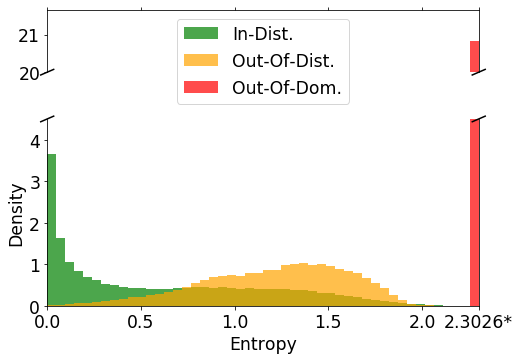
\includegraphics[width=.98 \textwidth]{sections/006_neurips2020/figures/entropy_CIFAR10.png}
        \caption{ID/OOD/OODom entropy}
    \end{subfigure}%  
    \begin{subfigure}[t]{0.33 \textwidth}
        \centering
        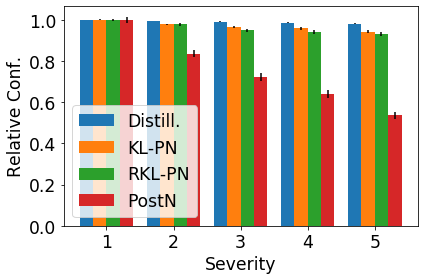
\includegraphics[width=.98 \textwidth]{sections/006_neurips2020/figures/shifts_CIFAR10_conf.png}
        \caption{Confidence under data shifts}
    \end{subfigure}%   
    \begin{subfigure}[t]{0.33 \textwidth}
        \centering
        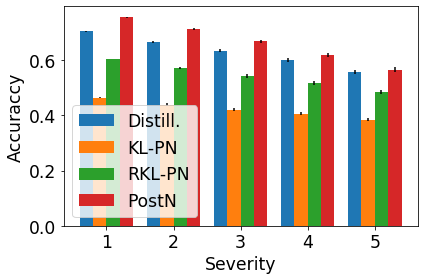
\includegraphics[width=.98 \textwidth]{sections/006_neurips2020/figures/shifts_CIFAR10_acc.png}
        \caption{Accuracy under data shifts}
    \end{subfigure}%   
    \caption{(a) shows entropy of the aleatoric distributions predicted by \oursacro on CIFAR10 (ID) and SVHN (OOD, OODom). The value $2.3026^*$ denotes the highest achievable entropy for 10 classes. \oursacro can easily distinguish between the three data types. (b) and (c) present averaged confidence and accuracy under 15 dataset shifts introduced by \cite{benchmarking_corruptions} on CIFAR10 with conv. architecture. On more severe perturbations (i.e. data further away from data distribution), \oursacro assigns higher epistemic uncertainty as desired. Baselines keeps same confidence even for less accurate predictions.}
    \label{cifar_shifts}
    %\vspace{-.5cm}
\end{figure}